\part{Reconnaissance d'un design pattern}

  \section{Reconnaître un design pattern à partir du code l'implémentant}

    J'ai poursuivi l'implémentation du code proposé, en implémentant
    le design pattern Factory pour la classe \texttt{EnchantedMazeGame}, et le résultat est disponible sur
    le dépôt Github associé à ce rendu
    \footnote{\url{https://github.com/aurelienshz/ii.2415-algo-prog/tree/master/tp2/mazegame/}}.

    Le diagramme de classes résultant de cette implémentation est le suivant :

    \begin{center}
      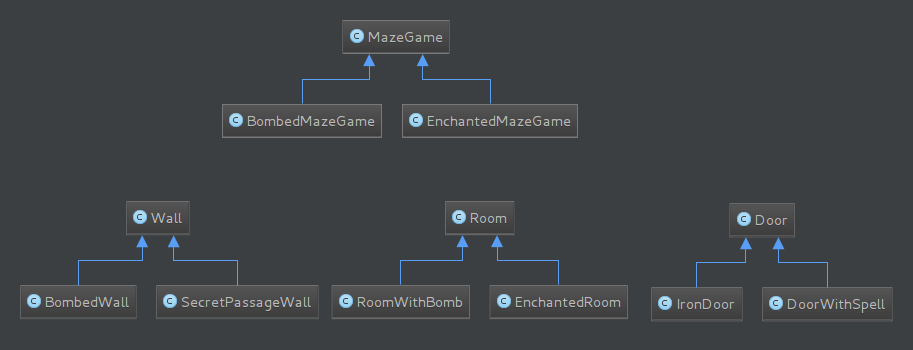
\includegraphics[width=13cm]{mazeClassDiagram}
    \end{center}

\newpage
  \section{Reconnaître un design pattern à partir d'un diagramme}

    Considérant le diagramme de classe ci-dessous :

    \begin{center}
      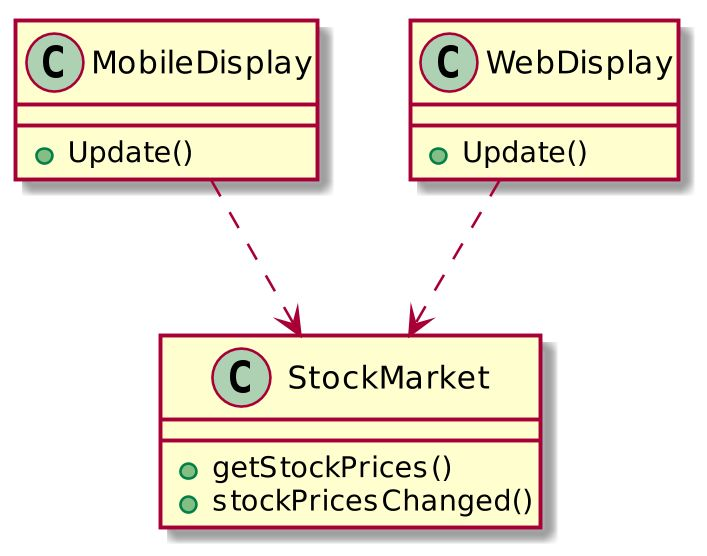
\includegraphics[width=8cm]{observerDiagram}
    \end{center}

    Le design pattern approprié à l'implémentation de ce diagramme de classes est le design pattern Observer :
    la class \texttt{MobileDisplay} et la classe \texttt{WebDisplay} seront les observateurs de la classe
    \texttt{StockMarket}, qui agira en observable.

  \section{Différencier deux patterns proches}

    Considérant les diagrammes de classes proposés pour le pattern A et le pattern B :
    \begin{itemize}
      \item le pattern A est le pattern "Strategy" ;
      \item le pattern B est le pattern "State".
    \end{itemize}

    Si ces deux design patterns se ressemblent par les interdépendances entre les classes qui les composent,
    ils se distinguent par leur emploi.

    En effet, le pattern "Strategy" sert
    à permettre de substituer différents algorithmes
    permettant de réaliser des traitements ayant les
    mêmes entrées et les mêmes sorties, de manière transparente.
    On utilise ce design pattern pour toutes les
    situations où l'on souhaite laisser les classes utilisatrices déterminer la stratégie à utiliser pour
    réaliser le traitement ; les classes implémentant l'interface qui décrit les entrées et les sorties
    sont totalement découplées et indépendantes, et ce sont les
    Il est typiquement
    très approprié pour la situation dans laquelle nous étions avec le TP n\textdegree1,
    où nous souhaitions comparer
    les performances de différents algorithmes de tri, pour un tableau initial toujours identique :
    on appellera alors toujours la même méthode, mais en l'informant de la \textit{stratégie} de tri
    à laquelle elle doit faire appel.

    Le pattern "State", quand à lui, sert à implémenter une machine à états. Il est utile dans les situations
    où le traitement des entrées successives entraîne des changements d'états dans l'application, qui
    entraîneront une variation des sorties (autrement dit, les entrées entraînent des changements d'états).
    Les différentes implémentations de l'interface définissant le traitement sont fortement couplées, et la
    classe \texttt{Context} se charge de les substituer l'une à l'autre lors des changements d'états.
    Il pourrait par exemple être approprié dans le cadre de l'implémentation d'un protocole réseau
    comme le HTTP, où la réception et l'envoi des différents messages d'établissement d'une connexion entraîne
    des changements d'état dans le programme chargé de l'établir (mais les entrées et les sorties sont
    toujours des paquets réseau).


\part{Refactorisation d'une application}

  \section{Commentaires}

    Le code proposé en exemple n'est ni générique, ni extensible.
    En effet, la méthode main est très fortement couplée avec toutes les autres classes de l'application
    (notamment \texttt{SelectionSort} et \texttt{BubbleSort}).
    Elle comporte beaucoup de code dupliqué, ce qui est très dangereux en termes de clarté et de
    maintenabilité du code.
    Enfin, elle n'autorise pas facilement l'ajout d'une nouvelle
    méthode de tri dont nous pourrions souhaiter mesurer les performances.

    Une approche de la solution pour éviter ce type de défaut a déjà été proposée lors du rendu du TP précédent.
    Cependant, cette approche justifie un peu de nettoyage, notamment à l'aide de l'un des designs patterns dont
    nous avons récemment eu connaissance.

  \section{Design patterns}

    Le design pattern le plus évident pour refactoriser le code proposé est le design pattern \textbf{Strategy} :
    la classe utilisatrice, responsable de tester les différents algorithmes de tri l'un après l'autre,
    s'adressera alors toujours à la même méthode, en lui passant en argument la stratégie à utiliser pour
    trier le tableau.

    Le design pattern Factory est également utile pour autoriser la classe chargée de lancer les mesures à
    instancier la classe chargée du tri de manière simple.

  \section{Refactorisation}

    Le résultat de la refactorisation du code écrit pour le TP1 est visible sur le dépôt Github associé
    à ce rendu\footnote{\url{https://github.com/aurelienshz/ii.2415-algo-prog}}.
    L'objectif général de cette refactorisation a été de rendre l'ensemble du design plus générique,
    en imposant l'interface que doivent implémenter les classes \texttt{Sorter}
    (par l'intermédiaire d'une classe abstraire \texttt{AbstractSorter}). Ainsi, il serait facile d'implémenter
    un nouvel algorithme de tri que nous pourrions souhaiter comparer à ceux déjà présents.
